\begin{scanpage}{0117}{100}
\begin{center}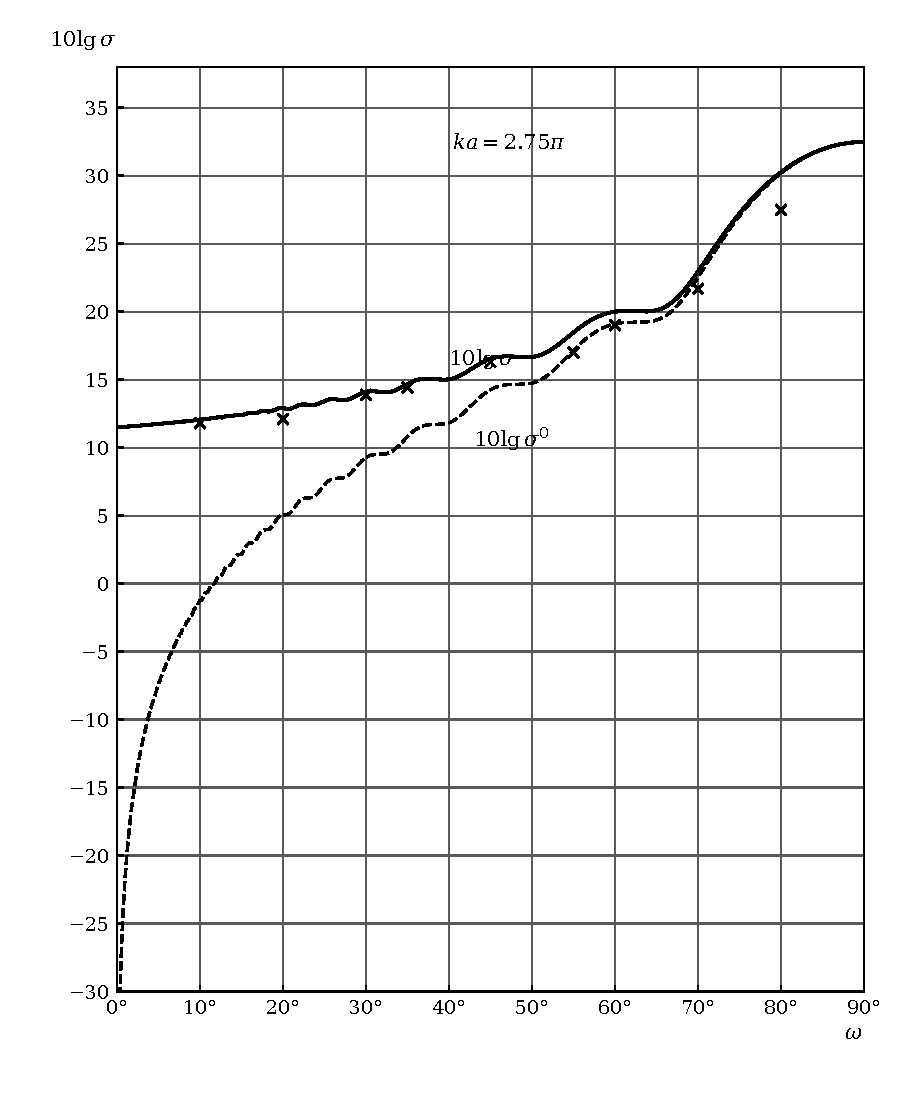
\includegraphics[width=.58\linewidth]{images/recreated/b-0117-fig32.pdf}

Figure 32. The effective scattering area of a finite cone as a function of the vertex angle.
\end{center}
\noindent\begin{minipage}[t]{.43\linewidth}\vspace{0pt}\centering
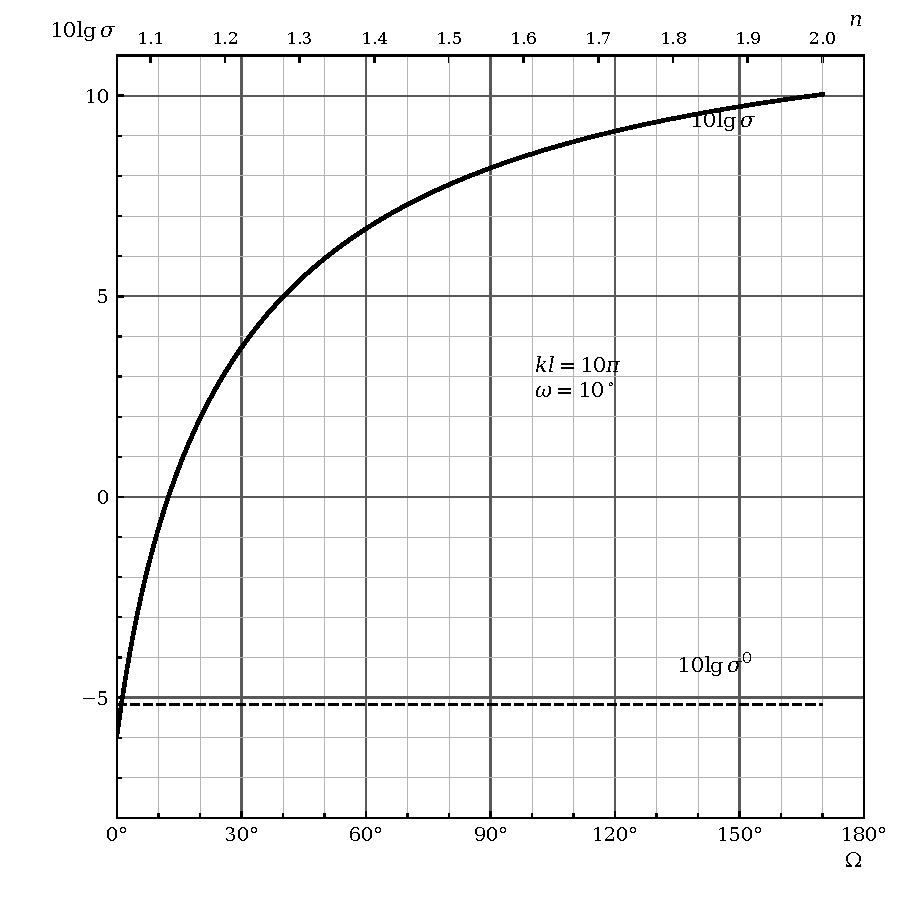
\includegraphics[width=.95\linewidth]{images/recreated/b-0117-fig33.pdf}

\raggedright Figure 33. The effective scattering area of a finite cone as a function of the shape of the shaded part.
\end{minipage}\hfill\begin{minipage}[t]{.53\linewidth}\vspace{0pt}
$z$ axis of the plane figure shown in Figure 34. Integrating the uniform part of the current, it is not difficult to show that the field scattered in the direction $\vartheta=\pi$ by the lateral surface of the truncated cone (Figure 35) is determined by the equation
\end{minipage}
\[\begin{aligned}E_x=-H_y=E_{0x}\biggl[&-\left(\frac i{4k}\operatorname{tg}^2\omega_1+\frac{a_1}2\operatorname{tg}\omega_1\right)e^{2ikl_1}\\&+\left(\frac i{4k}\operatorname{tg}^2\omega_1+\frac{a_2}2\operatorname{tg}\omega_1\right)e^{2ik(l_1+l_2)}\biggr]\frac{e^{ikR}}R.\end{aligned}\tag{17.16}\]
\end{scanpage}
